\section{Aufbau} 
Der Aufbau ist schematisch in Abbildung \ref{fig:Aufbau} dargestellt. 
Der optische Aufbau dieses Versuchs besteht aus einer 
Rb-Spektrallampe, zwei Sammellinsen, einem Interferenzfilter, 
einem Polarisationsfilter, einem $\sfrac{\lambda}{4}$-Plätchen und einem Photoelement. 
Die Sammellinsen werden verwendet um das Licht zu kollimieren und werden deshalb vor die Lampe 
und vor das Photoelement gestellt. Der Interferenz-,Polarisationsfilter und das 
$\sfrac{\lambda}{4}$-Plätchen werden in dieser Reihenfolge aufgestellt, damit genau das 
Rb-Spektrum ( $\lambda = \SI{794,8}{\nano\meter}$) herausgefilter wird und zirkular-polarisiert 
auf die Dampfzelle trifft. Das Licht aus der Dampfzelle wir kollimiert und auf das Photoelement 
fokusiert. Unter der Dampfzelle befindet sich eine Heizung, um für den richtigen Dampfdruck zu 
sorgen. Das Photoelement ist an ein Oszilloskop angeschlossen, um die entstehenden Ströme zu 
messen. Die Dampfzelle ist von drei Helmholzspulenpaaren umgeben. Zwei davon sind aufeinander 
aufgewickelt und erzeugen ein horizontales Feld (Sweep und Horizentalfeld-Spule). Das 
Erdmagnetfeld soll ausgeglichen werden, dabei sollte darauf geachtet werden, dass die 
Messapparatur in Nord-Süd-Richtung steht, damit das Erdmagnetfeld durch ein vertikales 
Magnetfeld kompensiert werden kann.
Die Sweepspule kann ein horizontales Modulationsfeld erzeugen. 
Damit kann dann die Resonanzstelle beobachtet werden. 
\begin{figure}
  \centering
  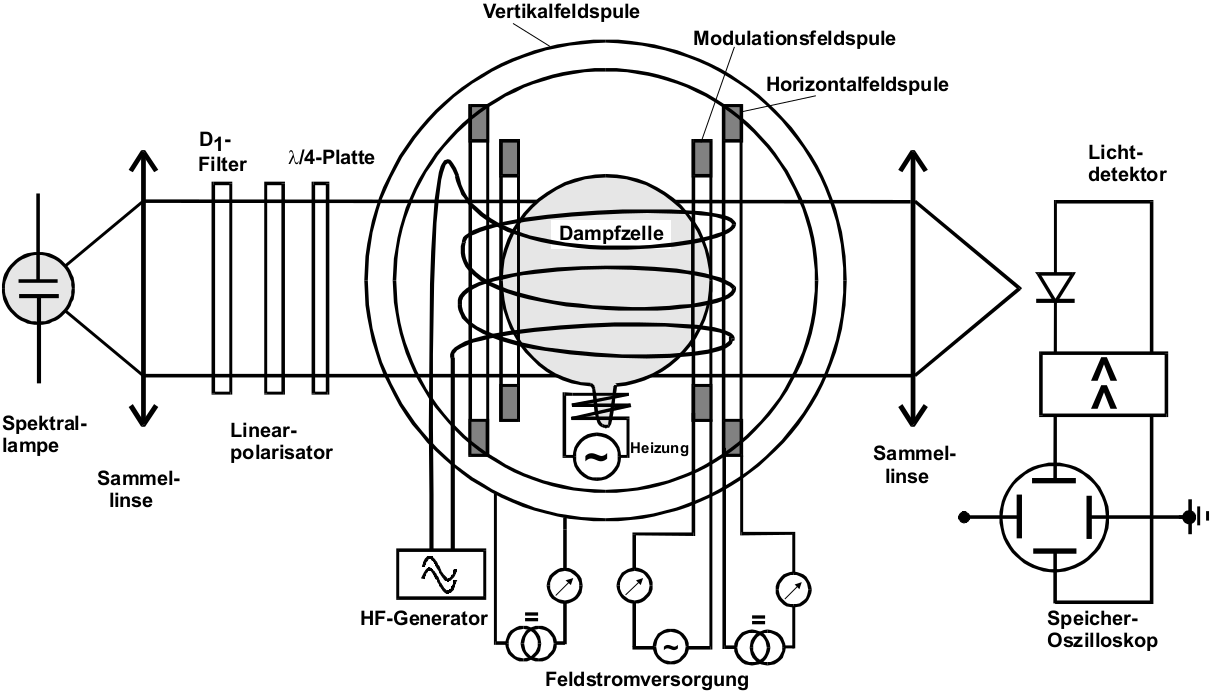
\includegraphics[height = 7cm]{pics/Aufbau.png}
  \caption{Schematische Darstellung des Aufbaus \cite{Anleitung}.}
  \label{fig:Aufbau}
\end{figure}

\section{Durchführung}
\label{sec:Durchführung}
Zuerst wird der Strahlengang für maximale Intensität eingestellt. Dann wird die Apparatur in 
Nord-Süd-Richtung gestellt und abgedeckt. Nun werden die Spulen eingeschaltet und auf Null 
eingestellt. Dann wird das Sweepfeld und das Signal des Photoelements auf das Ozilloskop gegeben [XY-Modus]. 
Jetzt 
sollte das Nullminimum aus der Theoriekurve \ref{fig:TheoK} zusehen sein, dieses soll mit 
der vertikalen Spule möglichst schmal eingestellt werden, um das Erdmagnetfeld zu kompensieren. 
Das Sweep- und Horizontalfeld stellen das RF-Feld da, dieses soll jetzt zwischen 
\SI{100}{\kilo\hertz} und \SI{1}{\mega\hertz} in Schritten von \SI{1}{\kilo\hertz} 
variiert werden. Dazu wird ein Sinus-Spannungsgenerator an das Kontrollgerät der RF-Spule angeschlossen. 
Nun wird das RF-Feld solange aufgedreht bis die Resonanz erscheint. Der Strom der durch die 
Spulen fließt kann dann am Potentiometer abgelesen werden, daraus kann dann später das 
Magnetfeld berechnet werden. Dabei treten Resonanzstellen für beide Isotope auf. 
Im Bereich ab \SI{200}{\kilo\hertz} muss ein zusätzliches horizontales Feld angelegt werden, um 
die Resonanzen in den Bereich des Sweepfeldes zu verschieben, der gerade auf dem 
Oszilloskop beobachtet werden kann. So kann die Theoriekurve für beide Isotope aufgenommen werden.
\newline 
Nun wird die Frequenz am Sinus-Spannungsgenerator auf \SI{100}{\kilo\hertz} eingestellt und mit 
Hilfe des Potentiometers am Konrtollgerät wird das Magnetfeld wieder auf die erste Resonanzstelle 
eingestellt. Jetzt wird ein zweiter Funktionsgenerator hinzugenommen und eine Rechteckspannung 
mit \SI{5}{\hertz} und \SI{5}{\volt} auf das Kontrollgerät der RF-SPule gegeben. Das Feld wird 
nun mit \SI{5}{\hertz} aus- und angeschaltet. Das Signal wird mit dem Signal des Photoelements 
auf das Oszilloskop gegeben. 
Beide Signale sollen jetzt im zeitlichen Verlauf dagestellt werden [YT-Modus]. 
Davon wird ein Bild aufgenommen.

